\documentclass[aspectratio=169]{beamer}
\usepackage{babel}
% \usepackage[german]{babel}

\usepackage{tikz, transparent, colortbl, listings, pgfplots}
\usepackage[export]{adjustbox}
\usepackage[skins,theorems]{tcolorbox}
 
\usetikzlibrary{automata,positioning}
\setbeamercovered{transparent}
\pgfplotsset{compat=1.18}
\tcbset{highlight math style={enhanced,colframe=red,colback=white,arc=0pt,boxrule=1pt}}

%
% Cited from Ausarbeitung/aspdoc.cls
%
\lstset{
    language=C++,
    basicstyle=\upshape\footnotesize\ttfamily,
    numbers=left,                   % where to put the line-numbers
    numberstyle=\tiny\color{gray},  % the style that is used for the line-numbers
    numbersep=5pt,                  % how far the line-numbers are from the code
    showstringspaces=false,
    frame=single,                   % adds a frame around the code
    rulecolor=\color{black},
    tabsize=2,                      % sets default tabsize to 2 spaces
    captionpos=b,                   % sets the caption-position to bottom
    breaklines=true,                % sets automatic line breaking
    breakatwhitespace=false,        % sets if automatic breaks should only happen at whitespace
    title=\lstname,                 % show the filename of files included with \lstinputlisting;
    keywordstyle=\color{blue},      % keyword style
    commentstyle=\color{dkgreen},   % comment style
    stringstyle=\color{mauve},      % string literal style
    escapeinside={\%*}{*)},         % if you want to add LaTeX within your code
}

% \lstset{
%     language=YAML,
%     basicstyle=\upshape\footnotesize\ttfamily,
%     numbers=left,
%     numberstyle=\tiny\color{gray},
%     numbersep=5pt,
%     showstringspaces=false,
%     frame=single,
%     rulecolor=\color{black},
%     tabsize=2,
%     captionpos=b,
%     breaklines=true,
%     breakatwhitespace=false,
%     title=\lstname,
%     keywordstyle=\color{blue},
%     commentstyle=\color{dkgreen},
%     stringstyle=\color{mauve},
%     escapeinside={\%*}{*)},
% }

% Useful Read:
% https://www.overleaf.com/learn/latex/Beamer

\title{Molecular Dynamics}
\subtitle{Group A}
\author{Haoyuan Ma \and Zhengying Zhao \and Anatoly Weinstein}
\date{31st of October 2025}

\newcommand{\framebackground}[2]{
    \begin{tikzpicture}
        \transparent{#1}
        \node[inner sep=0] at (current page.center) {
            
\includegraphics[height=\paperheight, right]{./media/tum-uhrenturm.png}
        };
        \transparent{1}
        \node[anchor=south, text width=\paperwidth, text height=1.5cm, draw=none, align=center] at (current page.south) {
            \insertpagenumber
        };
        \transparent{#2}
        \node[anchor=south, text width=\paperwidth, text height=1.5cm, draw=none, align=right] at (current page.south) {
            \small Haoyuan Ma, Zhengying Z, Anatoly W. \,\,
        };
    \end{tikzpicture}
}

\newcommand{\headerframe}{
    \usebackgroundtemplate{
        \framebackground{0.2}{1}
    }
}

\newcommand{\simpleframe}{
    \usebackgroundtemplate{
        \framebackground{0}{1}
    }
}

\newcommand{\blue}[1]{{\color{beamer@blendedblue} #1}}
\newcommand{\yellow}[1]{{\color[HTML]{AF8F10} #1}}
\newcommand{\gray}[1]{{\color[HTML]{8F8F8F} #1}}
\newcommand{\red}[1]{{\color[HTML]{FF5F5F} #1}}

\begin{document}

%
% Frame
%
\usebackgroundtemplate{\framebackground{0.2}{0}}
\begin{frame}
    \maketitle
\end{frame}

\simpleframe\begin{frame}{Wrapping up tech debt from Assignment 1: `App \& Core' Pattern}
    \centering
    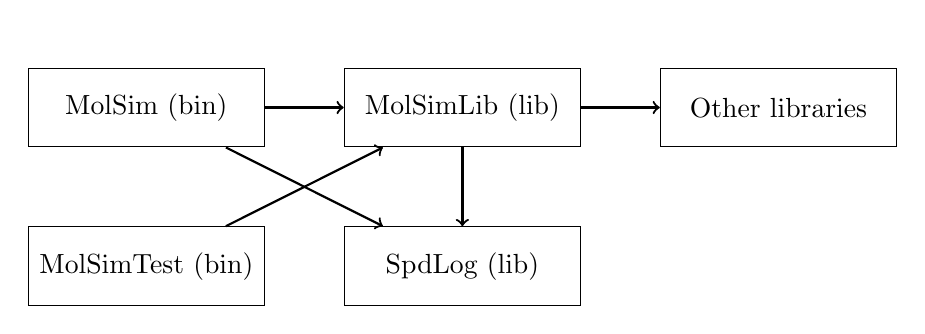
\begin{tikzpicture}[node distance=1cm and 1cm, minimum height=1cm, minimum width=3cm]
        \node[draw, rectangle] (bin) {MolSim (bin)};
        \node[draw, rectangle, below=of bin] (test) {MolSimTest (bin)};

        \node[draw, rectangle, right=of bin] (lib) {MolSimLib (lib)};
        \node[draw, rectangle, below=1cm of lib] (spdlog) {SpdLog (lib)};

        \node[draw, rectangle, right=of lib] (other) {Other libraries};

        \draw[->, thick] (test) -- (lib) node[midway, above] {};
        \draw[->, thick] (bin) -- (lib) node[midway, above] {};

        \draw[->, thick] (bin) -- (spdlog) node[midway, above] {};
        \draw[->, thick] (lib) -- (spdlog) node[midway, above] {};

        \draw[->, thick] (lib) -- (other) node[midway, above] {};
    \end{tikzpicture}

    \vspace{0.5cm}
    \begin{itemize}
        \item \blue{App `MolSim'} is executable that contains \blue{only interface-level logic}: argument parsing, simulation setup, etc.
        \item \blue{Core `MolSimLib'} is a library that contains \blue{the implementation}: particle simulations, etc.
    \end{itemize}
\end{frame}

\simpleframe\begin{frame}[fragile]{Wrapping up tech debt from Assignment 2: Caching Github CI builds}

    \begin{columns}
        \begin{column}{0.5\textwidth}
            Without Caching\footnotemark:

            \begin{itemize}
                \item \blue{2m 16s} Full Workflow Build
                \item \blue{2m 8s} CMake Build Step
            \end{itemize}
        \end{column}
        \begin{column}{0.5\textwidth}
            With Caching\footnotemark:

            \begin{itemize}
                \item \blue{43s} Full Workflow Build
                \item \blue{28s} CMake Build Step
                \item \blue{3s} Cache Retrieve
            \end{itemize}
        \end{column}
    \end{columns}

    \vspace{0.5cm}
    \begin{itemize}
        \item \blue{4x} performance speed up of CMake build!
    \end{itemize}

    % \footnotetext[1]{\href{https://github.com/Anatoly03/MolSim-WS25-GroupA/actions/runs/19469598810/job/55712979585}{Link to CI Run #72}}
    % \footnotetext[2]{\href{https://github.com/Anatoly03/MolSim-WS25-GroupA/actions/runs/19470075154/job/55714616480}{Link to CI Run #73}}
    \footnotetext[1]{CI Run \#72}
    \footnotetext[2]{CI Run \#73}
\end{frame}

\simpleframe\begin{frame}[fragile]{Adding YAML Support}

    \begin{lstlisting}
name: Simple Setup

config:
  delta_time: 0.14
  total_time: 100
  output: OutputFile
  output_interval: 20

particles:
  - position: [0.0, 0.0, 0.0]
    velocity: [0.01, 0.0, 0.0]
    mass: 1.0
\end{lstlisting}

    \blue{Extensible} and \blue{human-readable} configuration format!
\end{frame}

\simpleframe\begin{frame}[fragile]{Adding YAML Support}

    \begin{lstlisting}
name: Cuboid and Sun

particles:
  cuboid:
    type: cuboid
    n: [40, 8, 1]
    position: [0.0, 0.0, 0.0]
    velocity: [0.0, 0.0, 0.0]
    mass: 1.0
    sigma: 1.0
    brownian_sigma: 0.1
  sun:
    position: [19.0, 16.0, 0.0]
    velocity: [0.0, -10.0, 0.0]
    mass: 1.0
\end{lstlisting}
\end{frame}

\simpleframe\begin{frame}{Our Weeks' Toughest Challenge: Circular Dependencies}
    \centering
    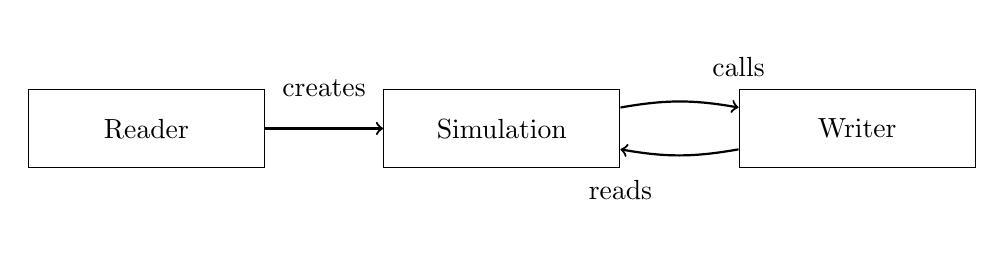
\begin{tikzpicture}[node distance=1cm and 1.5cm, minimum height=1cm, minimum width=3cm]
        \node[draw, rectangle] (r) {Reader};
        \node[draw, rectangle, right=of r] (s) {Simulation};
        \node[draw, rectangle, right=of s] (w) {Writer};

        \draw[->, thick] (r) -- (s) node[midway, above] { creates };
        \draw[->, thick] (s) to[bend left=10] (w) node[above] { calls };
        \draw[->, thick] (w) to[bend left=10] (s) node[below] { reads };
    \end{tikzpicture}

    \vspace{0.5cm}
    \begin{itemize}
        \item Circular dependency between \blue{Writer} and \blue{Simulation}!
        \item Forward declaration of no help because we need full type information.
        \item Refactoring the entire codebase proved more lethal in discarded commits than our magic trick (next slide).
    \end{itemize}
\end{frame}

\simpleframe\begin{frame}{Our Weeks' Toughest Challenge: Circular Dependencies}
    \vspace{0.5cm}
    \begin{itemize}
        \item \blue{Our Fix:} Use \yellow{functional, data-driven callbacks} to break the circular dependency!
        \item This needs to be optimized. We are not happy with this design, but it works as a short-term solution.
    \end{itemize}

    \centering
    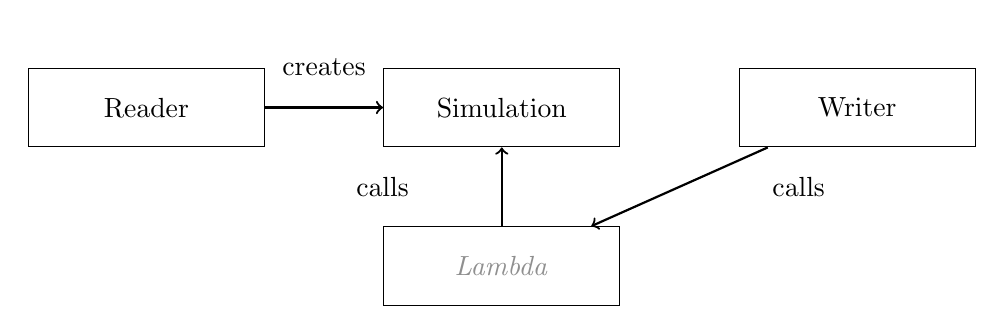
\begin{tikzpicture}[node distance=1cm and 1.5cm, minimum height=1cm, minimum width=3cm]
        \node[draw, rectangle] (r) {Reader};
        \node[draw, rectangle, right=of r] (s) {Simulation};
        \node[draw, rectangle, right=of s] (w) {Writer};
        \node[draw, rectangle, below=of s] (cb) {\gray{\textit{Lambda}}};

        \draw[->, thick] (r) -- (s) node[midway, above] { creates };
        \draw[->, thick] (cb) -- (s) node[midway, left] { calls };
        \draw[->, thick] (w) -- (cb) node[midway, right] { calls };
    \end{tikzpicture}
\end{frame}


\simpleframe\begin{frame}{Our physics is weird – Cuboid Example Case Study}
    \begin{columns}
        \begin{column}{0.5\textwidth}
            \begin{figure}
                \centering
                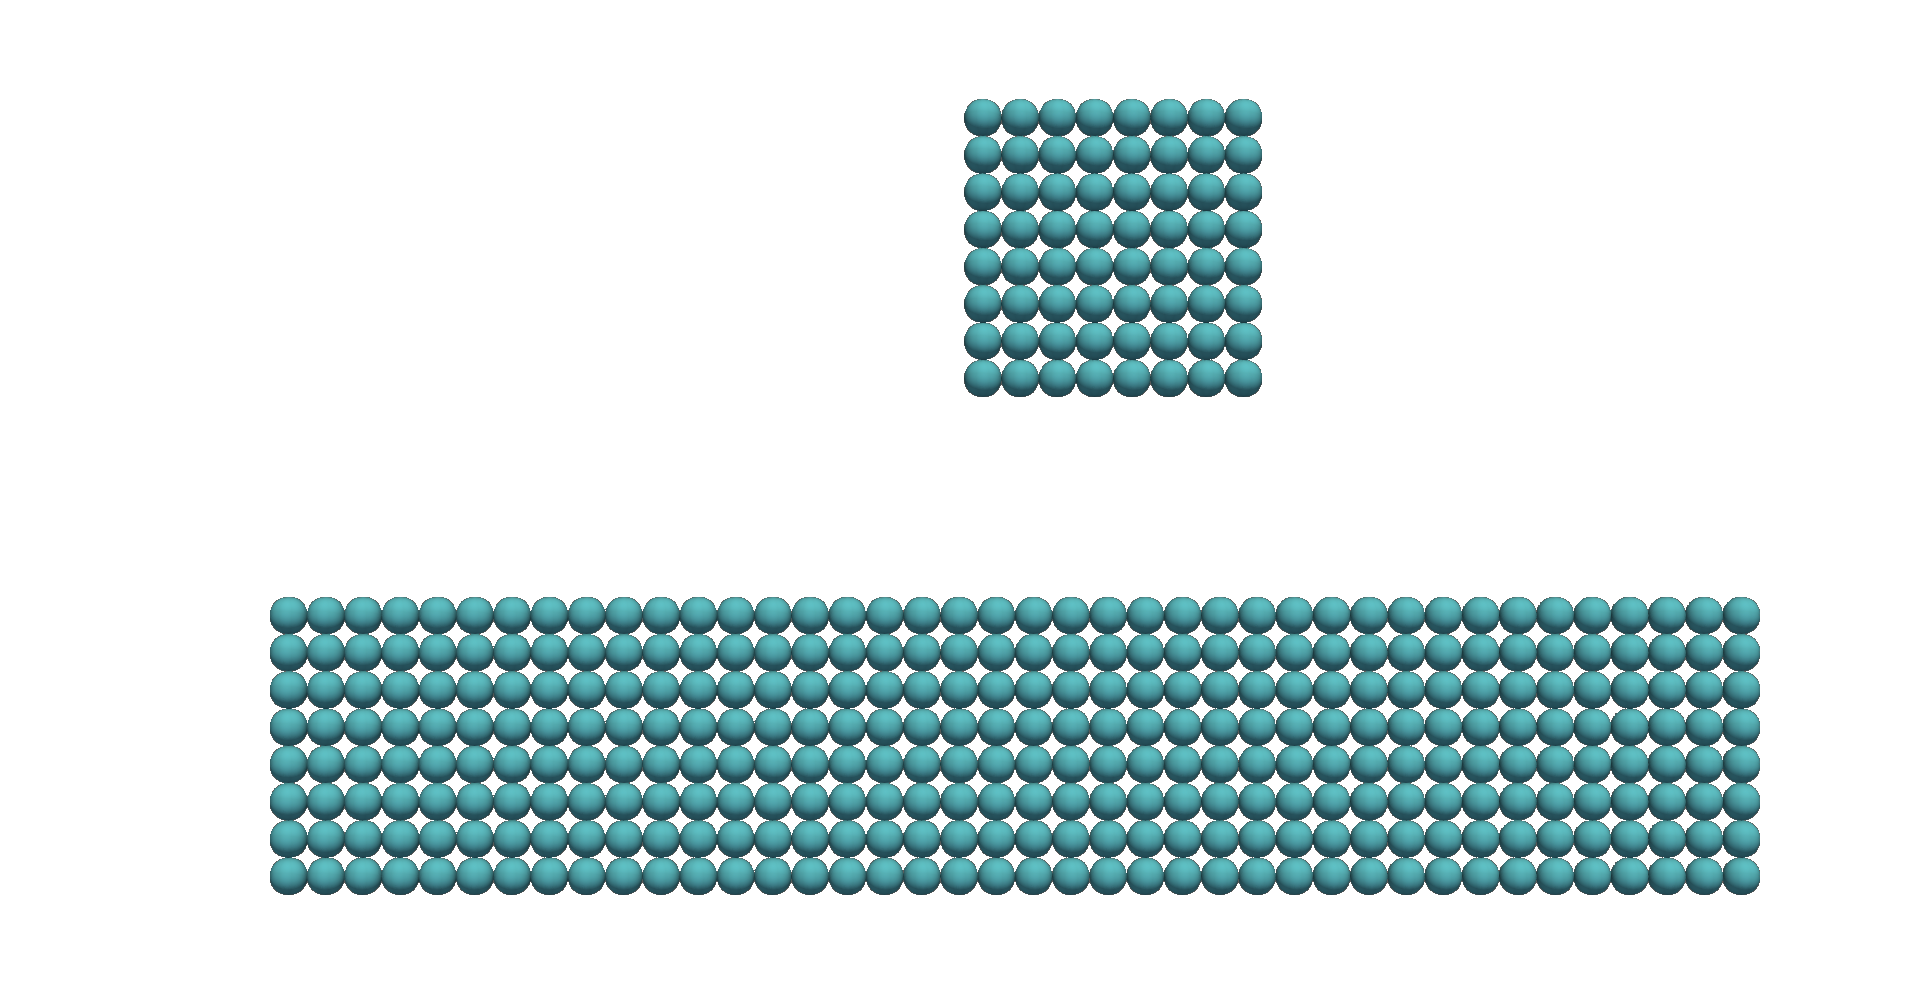
\includegraphics[width=0.6\textwidth]{media/w3-cuboid1.png}
                \caption{Starting configuration}
            \end{figure}
        \end{column}
        \begin{column}{0.5\textwidth}
            \begin{figure}
                \centering
                
\includegraphics[width=0.6\textwidth]{media/w3-cuboid2.png}
                \caption{After 20 ticks}
            \end{figure}
        \end{column}
    \end{columns}
    
    \vspace{-0.5cm}
    \begin{figure}
        \centering
        
\includegraphics[width=0.3\textwidth]{media/w3-cuboid3.png}
        \caption{After 40 ticks}
    \end{figure}
\end{frame}

\headerframe\begin{frame}{That's it – for now, at least}{Shaw! We thank you for your attention!}
    \begin{center}
        \begin{figure}
        \centering
        
\includegraphics[width=0.35\textwidth]{media/shaw.png}
    \end{figure}
    \end{center}
\end{frame}

\end{document}
